% !TeX TXS-program:compile = txs:///pdflatex/[--shell-escape]

\documentclass[a4paper]{article}
\usepackage{fullpage}
\usepackage[spanish]{babel}

\usepackage[default]{lato}  %% Option 'sfdefault' only if the base font of the document is to be sans serif
\usepackage[scaled=.9]{noto-mono} %% Change default mono font
\usepackage[T1]{fontenc}
\usepackage[utf8]{inputenc}

\usepackage{graphicx}
\usepackage[dvipsnames]{xcolor}
\usepackage{colortbl}

% \usepackage{palatino}

\usepackage{fontawesome}

% setlists (itemize, enumerate) with customized icons
\usepackage[shortlabels]{enumitem}

\newcommand{\usageitem}[1]{%
  \item[%
    {\makebox[2em]{\strut #1}}%
  ]
}

%% Ajustar interlineado entre párrafos a una línea en blanco
\setlength{\parskip}{2mm}

\usepackage{enumitem}

% Roman numbers for section
\renewcommand{\thesection}{\Roman{section}} 
\renewcommand{\thesubsection}{\thesection.\Arabic{subsection}}

\usepackage{url}
%%% PDF file metadata

%%% Customized colors for this document
\definecolor{darkred}{rgb}{0.5,0,0}
\definecolor{darkgreen}{rgb}{0,0.5,0}
\definecolor{darkblue}{rgb}{0,0,0.5}

% Colored boxes for information corners
\usepackage{tcolorbox}% http://ctan.org/pkg/tcolorbox

% Caja azul con título para información, explicaciones extra y detalles
% Icons: \faInfoCircle \faBook \faBookmark
\newtcolorbox{mybluebox}[1]{colback=darkblue!5!white,colframe=darkblue!75!black,
                            fonttitle=\normalfont,title=#1}
                            
% Caja verde para comentarios adicionales
% Icons: \faComment \faCrosshairs
\newtcolorbox{mygreenbox}[1]{colback=darkgreen!5!white,colframe=darkgreen!75!black,
                             fonttitle=\normalfont,title=#1}
                             
% Caja roja con título para posibles problemas explicaciones extra y detalles
% Icons: \faExclamationCircle \faBomb
\newtcolorbox{myredbox}[1]{colback=darkred!5!white,colframe=darkred!75!black,
                           fonttitle=\normalfont,title=#1}
                       
\usepackage{enumitem}% http://ctan.org/pkg/enumitem

\usepackage{minted}
% \usepackage{tcolorbox}
% \tcbuselibrary{minted,skins}
% 
% \newtcblisting{bashcode}{
%   listing engine=minted,
%   colback=bashcodebg,
%   colframe=black!70,
%   listing only,
%   minted style=colorful,
%   minted language=bash,
%   minted options={linenos=true,texcl=true},
%   left=1mm,
% }
% \definecolor{bashcodebg}{rgb}{0.85,0.85,0.85}
% 
% \newtcblisting{pycode}{
%   listing engine=minted,
%   colback=pycodebg,
%   colframe=black!70,
%   listing only,
%   minted style=colorful,
%   minted language=python,
%   minted options={linenos=true,texcl=true},
%   left=1mm,
% }
% \definecolor{pycodebg}{rgb}{0.85,0.85,0.85}

\usepackage[pdftex]{hyperref}

\definecolor{darkred}{rgb}{0.5,0,0}
\definecolor{darkgreen}{rgb}{0,0.5,0}
\definecolor{darkblue}{rgb}{0,0,0.5}

\hypersetup{
    pdftoolbar=true,	%Shows Adobe Acrobat toolbar
    pdfmenubar=true,	%Shows Adobe Acrobat menu
    pdftitle={AI - Bloque II - Práctica - 2020},
    pdfauthor={Juan González, Felipe Ortega},
    pdfcreator={GSyC, ETSIT},
    pdfproducer={PDFLaTeX},
    pdfsubject={AI - Evaluación - Práctica - 2020},
    pdfnewwindow=true,  %links open in new window
    colorlinks=true,    %false: boxed links; true: coloured links
    linkcolor=darkred,
    citecolor=darkgreen,
    urlcolor=darkblue
}

\begin{document}
	

\includegraphics[width=2.5cm]{gsyc-logo-small.png} \hspace{8cm} 
\includegraphics[width=4cm]{URJClogo.png}

%--- Heading metadata
\begin{center}
 \LARGE{\textbf{Evaluación Bloque II (Práctica)}}
 \smallskip
 
 \large{\textbf{Arquitectura de Internet}}
 
 \large{Grado en Ing. Sistemas Audiovisuales y Multimedia}
 
 \large{ETSIT, URJC}
 \smallskip
 
 \large{\underline{\today}}
\end{center}
\bigskip

\hrule
\medskip

\setlist[itemize]{leftmargin=12mm}

\begin{itemize}[leftmargin=0.8cm,itemsep=6pt,topsep=6pt]
  \usageitem{\faSend} \textbf{Envío}: El envío se realizará a través del espacio de entrega
  habilitado en el apartado \textit{Evaluación} de la página de la asignatura en Aula Virtual.
	
  \usageitem{\faWrench} \textbf{Herramientas software}: Utiliza NetGUI, Wireshark así como las herramientas
  Linux que se han ido introduciendo en las Prácticas 0 a 3 para contestar las preguntas de
  cada apartado. 
  
  \usageitem{\faFileO} \textbf{Formato}: Puedes enviar tus respuestas en un fichero de procesador de textos (LibreOffice
  u OpenOffice) o en formato PDF. También es válido componer un documento con una herramienta
  de notas para tables, siempre que el envío se realice \textbf{en formato PDF}.
  
  \usageitem{\faExclamationCircle} \textbf{Advertencia}: Incluye claramente en el documento
  de tu respuesta tus datos personales, así como \textbf{toda la información solicitada} en
  cada pregunta (pantallazos, comandos, justificaciones, etc.). De lo contrario, la respuesta
  no puntuará.
  
  \usageitem{\faCalendar} \textbf{Fecha tope de entrega}: \textbf{\underline{Domingo, 17 de mayo de 2020}}.
\end{itemize}

\medskip
\hrule
%--- End of heading metadata

\bigskip

\section{Protocolos y Ethernet}
\label{sec:protocolos-eth}

\textbf{Abre} el fichero de captura \href{file://captura1.cap}{captura1.cap} con \href{https://www.wireshark.org/}{Wireshark} y \textbf{responde} a las siguientes preguntas:

\begin{enumerate}
	\item ¿Cuantas tramas se han capturado en total?
	
	\item Accede a la trama capturada a los \textbf{184.088902} segundos. Indica qué 
	\textbf{protocolos} se usan y \textbf{a qué nivel} de la \textbf{arquitectura TCP/IP} corresponden.
	
	\item Seguimos con \textbf{la misma trama} anterior, capturada a los \textbf{184.088902} segundos. Responde a las siguientes preguntas:
	
	\begin{enumerate}[label*=\arabic*.]
		\item ¿Cuantos bytes se envía por el cable físico? (Sin contar el preámbulo y el CRC)    
		\item ¿Y contando el CRC?    
		\item ¿Cuantos bytes tiene la cabecera del \textbf{protocolo Ethernet}?    
		\item ¿Cuántos bytes tiene la cabecera del \textbf{protocolo IP}? (si lo usa)  
		\item ¿Cuántos bytes tiene la cabecera del \textbf{protocolo TCP}? (si lo usa)  
		\item ¿Cuántos bytes tiene la parte del \textbf{protocolo HTTP}? (si lo usa)  
	\end{enumerate}

	\item Usando la \textbf{misma trama} anterior, responde las siguientes preguntas:
	
	\begin{enumerate}[label*=\arabic*.]
		\item ¿Cuál es la \textbf{dirección física} de la máquina que recibe la trama?  
		\item ¿Cuá es la \textbf{dirección física} de la máquina que envía la trama?  
		\item ¿Cuál es el valor del campo \texttt{Type} de esta trama Ethernet?
	\end{enumerate}

    \item \textbf{Analiza} todas las tramas y escribe todos los protocolos diferentes 
    que veas que se están usando, y clasifícalos según los niveles de la 
    \textbf{arquitectura TCP/IP}.
    
    \item Analiza la trama número 32:
    
    \begin{enumerate}[label*=\arabic*.]
    	\item ¿Cuántos dato útiles (bytes) se transportan en el protocolo de último nivel?  
    	\item ¿Qué mensaje se está enviando? 
    \end{enumerate}
    
	
\end{enumerate}

%%%---------------------------------------------- 

\section{Direcciones IP}
\label{sec:ips}

\begin{enumerate}
	\item Arranca \textbf{Netgui} y construye esta \textbf{subred} formada por 3 PCs.
    \smallskip
    
    \begin{myredbox}{\faExclamationCircle~~\textbf{Nota Importante}}
    	El \textbf{nombre de los PCs} debe debe terminar con \textbf{un guión} 
    	seguido de \textbf{tus iniciales}.  
    	Así, un estudiante que se llame \texttt{Antonio González Márquez} deberá 
    	añadir el sufijo \texttt{-agm} a los nombres de los PCs, tal y como se muestra
    	en la Figura~\ref{fig:label-pcs}.
    \end{myredbox}
    \medskip
	
	\begin{figure}
		\begin{center}
			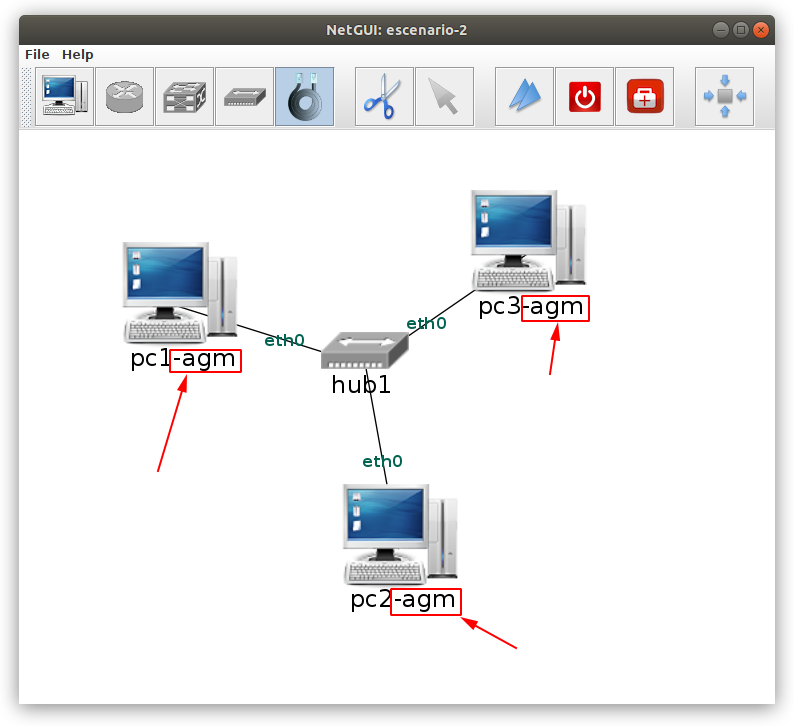
\includegraphics[width=10cm]{ip-01.png}
		\end{center}
		\caption{Ejemplo de nombrado de los PCs para la realización de este
		ejercicio práctico.}
	    \label{fig:label-pcs}
	\end{figure}

	Toma un \textbf{pantallazo} del escenario y adjúntalo como respuesta a esta pregunta.
	
	\item \textbf{Configura} las direcciones IP de las \textbf{tres máquinas} para que 
	pertecezcan a la  
	misma subred.
	\smallskip
	
	\begin{myredbox}{\faExclamationCircle~~\textbf{Nota Importante}}
		El primer byte de todas las IP debe estar formado  
		por los \textbf{dos primeros dígitos de tu DNI}, y el segundo byte por los dos siguientes.  El resto  
		de bytes y la máscara de subred puede ser las que tú elijas, pero compatibles con que los
		ordenadores pertenezcan a la misma subred. Por ejemplo, si el DNI de Antonio González 
		Márquez es \texttt{12345678W}, las direcciones IP debe ser de la forma \texttt{12.34.x.x}.
	\end{myredbox}
	\smallskip 
	
	\textbf{Rellena} esta tabla con la información, y \textbf{configura} los PCs para que tengan esas \textbf{direcciones IP} (de manera no persistente).
	\medskip
	
	\bgroup
	\def\arraystretch{1.5}%  1 is the default, change whatever you need
	\begin{tabular}{|l|l|}
		\hline 
		\textbf{Nombre PC}& \textbf{Dirección IP} \\ 
		\hline 
		pc1-xxx &  \\ 
		\hline 
		pc2-xxx &  \\ 
		\hline 
		pc3-xxx &  \\ 
		\hline 
	\end{tabular} 
    \egroup
    \medskip
    
    \item \textbf{Completa} la siguiente tabla, indicando los \textbf{comandos} que has 
    empleado para \textbf{configurar} cada máquina.
    \medskip
    
    \bgroup
    \def\arraystretch{1.5}%  1 is the default, change whatever you need
    \begin{tabular}{|l|l|}
    	\hline 
    	\textbf{Nombre PC}& \textbf{Comando} \\ 
    	\hline 
    	pc1-xxx &  \\ 
    	\hline 
    	pc2-xxx &  \\ 
    	\hline 
    	pc3-xxx &  \\ 
    	\hline 
    \end{tabular} 
    \egroup
    \medskip
	
	\item \textbf{Comprobación} de las direcciones IP: Deberás usar el comando necesario para que aparezca en el terminal la \textbf{informaión de la configuración} de cada PC. Adjunta \textbf{un pantallazo} de \textbf{cada terminal}, con esa información. Para el ejemplo de nuestro  estudiante \texttt{Antonio González Márquez}, la información de configuración del PC1 
	sería como muestra la Figura~\ref{fig:ips}.
	
	\begin{figure}
		\begin{center}
			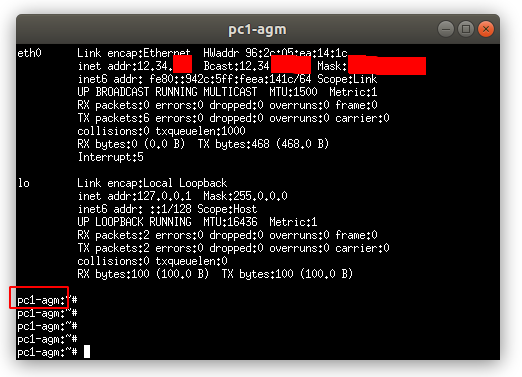
\includegraphics[width=13cm]{ip-02.png}
		\end{center}
		\caption{Ejemplo de pantallazo con la información de direccionamiento IP que se debe
			incluir en la respuesta del apartado 3 (Se ha eliminado la información importante).}
		\label{fig:ips}
	\end{figure}
 
    \item \textbf{Comprueba} efectivamente que hay \textbf{conectividad} entre la máquina 
    PC1 y PC2.
    
    \begin{enumerate}[label*=\arabic*.]
    	\item ¿Qué comando usas para ello?  
    	\item Crea un \textbf{pantallazo} de la terminal mostrando que efectivamente hay conectividad.
    \end{enumerate}

    \item Sitúate en \textbf{PC3} e inicia la \textbf{captura el tráfico} que hay en la red. El resultado se almacenará en un
    fichero llamado \texttt{captura1-xxx.cap} donde \texttt{xxx} es el sufijo que has usado anteriormente con tus iniciales. Escribe el \textbf{comando completo} que has usado para realizar la captura.
    
    \item Desde PC1 usa el comando ping contra PC2, para que le envíe 3 mensajes, y termina la captura del tráfico. Muestra un pantallazo del terminal de PC1 con los resultados del comando \texttt{ping}.
    
    \item Abre con \textbf{Wireshark} la captura que has realizado y saca un \textbf{pantallazo} donde se vean claramente  
    todos los paquetes que han circulado por la subred.
	    
\end{enumerate}


%%%------------------------------------------

\section{Enrutamiento}
\label{sec:routing}

\begin{enumerate}
	\item Arranca \textbf{NetGUI} y crea un \textbf{escenario} como el que se muestra en 
	la Figura~\ref{fig:router1}, usando la nomenclatura  definida en la parte anterior. Es decir, añade a \textbf{cada PC} un \textbf{sufijo con tus iniciales}, y lo mismo para los \textbf{\textit{routers}}.  En el caso de nuestro estudiante \texttt{Antonio González Márquez}, el escenario quedaría como muestra la Figura~\ref{fig:router1}.
					
	\begin{figure}
		\begin{center}
			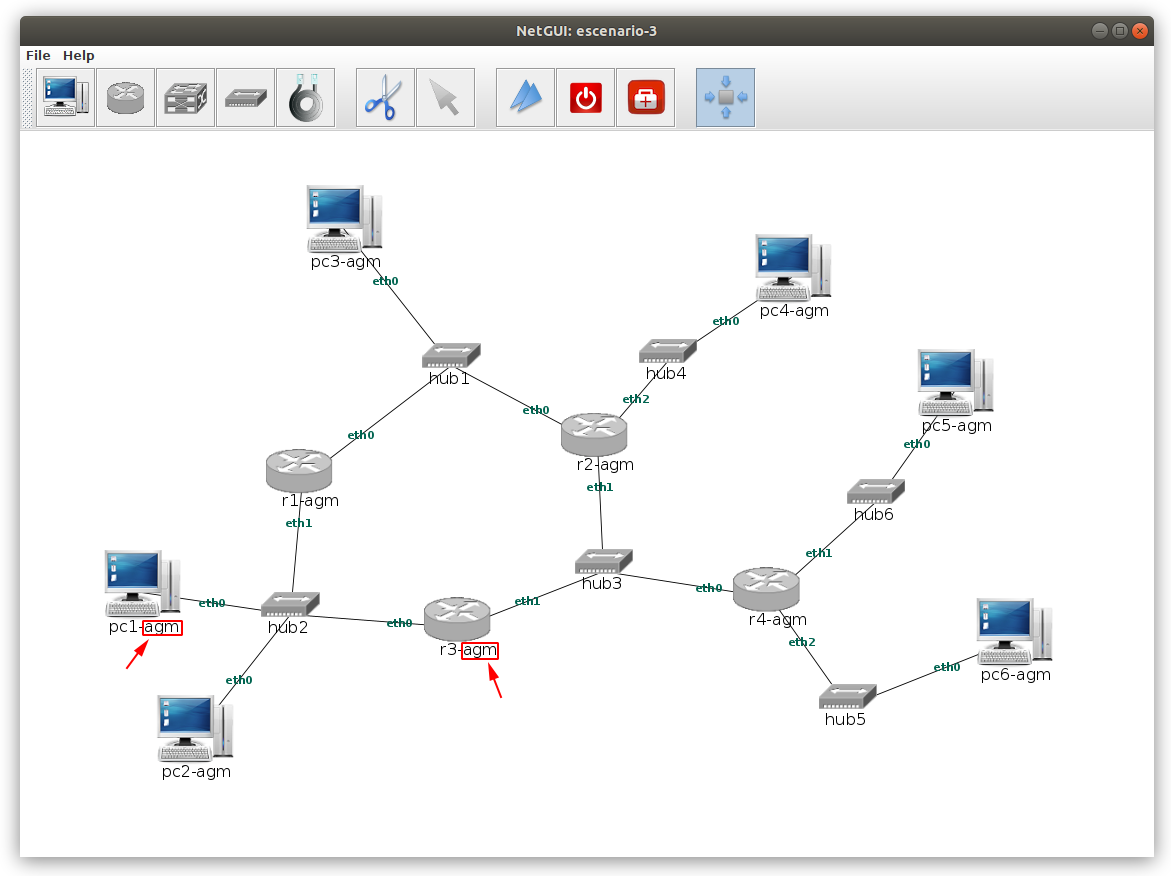
\includegraphics[width=13cm]{ruter-01.png}
		\end{center}
		\caption{Ejemplo de pantallazo con el nombre que se debe dar a los routers en el escenario
		propuesto en esta parte.}
		\label{fig:router1}
	\end{figure}

	\begin{myredbox}{\faExclamationCircle~~\textbf{Nota Importante}}
		Respeta la numeración tanto en los PCs como en los \textit{routers} (es indiferente 
		en los hubs).
	\end{myredbox}
	\smallskip 

    Obtén un \textbf{pantallazo} de tu escenario e inclúyelo en el documento con las
    soluciones.
    
    \item ¿Cuantas subredes hay en este escenario?
    
    \item Crea una \textbf{tabla} las \textbf{direcciones IP de las subredes} y sus \textbf{máscaras}. Define las que tu quieras, \textbf{PERO}  
	deben cumplir con la misma \textbf{restricción} que en la sección~\ref{sec:ips}: debes usar 
	los \textbf{4 primeros dígitos} de tu \textbf{DNI} para los 2 primeros bytes 
	de las IPs. Así, para el caso del estudiante \texttt{Antonio González Márquez}, todas
	las IPs comienzan por \texttt{12.34.x.x}.
	
	\bgroup
	\def\arraystretch{1.5}%  1 is the default, change whatever you need
	\begin{tabular}{|c|c|}
		\hline 
		\textbf{Dirección de subred}& \textbf{Máscara de subred} \\ 
		\hline 
		$\dots$ & $\dots$ \\ 
		\hline 
		$\dots$ & $\dots$ \\ 
		\hline 
		$\dots$ & $\dots$ \\ 
		\hline 
	\end{tabular} 
	\egroup
	\medskip
	
	\item Asigna a todas las interfaces de los PCs y los rúters una dirección IP. Escríbelo
	en la siguiente tabla:
	\medskip
	
	\bgroup
	\def\arraystretch{1.5}%  1 is the default, change whatever you need
	\begin{tabular}{|l|c|c|}
		\hline 
		\textbf{Nombre de máquina} & \textbf{IP} & \textbf{Interfaz} \\ 
		\hline 
		\texttt{pc1-xxx} & & \texttt{eth0} \\ 
		\hline 
		\texttt{pc2-xxx} & & \texttt{eth0} \\ 
		\hline 
		\texttt{pc3-xxx} & & \texttt{eth0} \\ 
		\hline 
		\texttt{pc4-xxx} & & \texttt{eth0} \\ 
		\hline 
		\texttt{pc5-xxx} & & \texttt{eth0} \\ 
		\hline 
		\texttt{pc6-xxx} & & \texttt{eth0} \\ 
		\hline 
		\texttt{r1-xxx} & & \texttt{eth0} \\ 
		\hline 
		\texttt{r1-xxx} & & \texttt{eth1} \\ 
		\hline 
		\texttt{r2-xxx} & & \texttt{eth0} \\ 
		\hline 
		\texttt{r2-xxx} & & \texttt{eth1} \\ 
		\hline 
		\texttt{r2-xxx} & & \texttt{eth2} \\ 
		\hline 
		\texttt{r3-xxx} & & \texttt{eth0} \\ 
		\hline 
		\texttt{r3-xxx} & & \texttt{eth1} \\ 
		\hline
		\texttt{r4-xxx} & & \texttt{eth0} \\ 
		\hline 
		\texttt{r4-xxx} & & \texttt{eth1} \\ 
		\hline 
		\texttt{r4-xxx} & & \texttt{eth2} \\ 
		\hline 
	\end{tabular} 
	\egroup
	\medskip
	
	\item Para configurar las direcciones IP de forma persistente, ¿Qué fichero de 
	configuración hay que usar?  
	
	\item ¿Qué comando hay que utilizar para hacer que los cambios sean efectivos?
	
	\item \textbf{Configura} de forma \textbf{persistente} las IPs de \textbf{TODAS} las máquinas,  tanto de los PCs como de los rúters. Escribe para cada máquina el \textbf{contenido del fichero de configuración} (el indicado en la pregunta 5)
	
	\item Una vez configuradas sólo las direcciones IP (todavía no están las tablas de enrutamiento), contesta a las siguientes preguntas:
	
	\begin{enumerate}[label*=\arabic*.]
		\item ¿Existe conectividad entre \texttt{pc1} y \texttt{pc2}?  
		\item ¿Existe conectividad entre \texttt{pc1} y \texttt{pc6}?
	\end{enumerate}
    \smallskip
    
    \item \textbf{Configura} de forma \textbf{persistente} la \textbf{tabla de enrutamiento} de \textbf{pc1} para que se pueda conectar con \textbf{pc3} y que los paquetes destinados a máquinas de otras subredes vayan a través del \textbf{\textit{router} r3}. Escribe el contenido del
    fichero de configuración.
    
    \item \textbf{Configura} de forma \textbf{persistente} la tabla de enrutamiento de \textbf{pc3} para que exista conectividad con \textbf{pc1}. Escribe el fichero de configuración.
    
    \item \textbf{Configura} las tablas de encaminamiento necesarias para que haya conectividad entre \texttt{pc1} y \texttt{pc6}. Los paquetes de \texttt{pc1} a \texttt{pc6} deben seguir la ruta \texttt{pc1} $\rightarrow$\texttt{r1} $\rightarrow$ 
    \texttt{r2} $\rightarrow$ \texttt{r4} $\rightarrow$ \texttt{p6}.  Y los
    paquetes de pc6 a pc1 deben seguir esta otra: \texttt{pc6} $\rightarrow$ \texttt{r4} 
    $\rightarrow$ \texttt{r3} $\rightarrow$ \texttt{pc1}. Escribe los \textbf{ficheros de configuración} de las máquinas que hayas modificado para lograrlo
    
    \item \textbf{Ejecuta} el comando \texttt{traceroute} en \texttt{pc1} con destino \texttt{pc6}. Toma un \textbf{pantallazo} del resultado.
    
    \item Ejecuta el comando \texttt{traceroute} en \texttt{pc6} con destino \texttt{pc1}. Toma un \textbf{pantallazo} del resultado
    
    \item Al ejecutar el traceroute anterior, ¿Se obtienen las IPs de los dos rúters intermedios? En caso de que no sea así, ¿Qué modificación debes realizar para que sí aparezcan?
    
    \item Lanza una captura de tráfico desde \texttt{r2(eth1)} en el fichero \texttt{captura2-xxx.cap} 
    donde \texttt{xxx} es el  
    sufijo con tus iniciales. \textbf{Ejecuta} el comando \texttt{traceroute} desde \texttt{pc1} a \texttt{pc6}. Abre la captura con  
    \textbf{Wireshark} y responde a las siguientes preguntas:

\end{enumerate}





  
%8.1: 
%
%9. 
%
%10.   
%15.1. ¿Cuantos paquetes se han capturado?  
%15.2. Indica cuál es el TTL de cada uno de ellos




\end{document}

